\documentclass[
  accentcolor=tud1c,	% Color theme for TUD corporate design
  colorbacktitle,		% Titlepage has colored background for title area
  inverttitle,			% Font color of title on titlepage is inverted
  german,
  twoside
]{tudexercise}

\usepackage[ngerman]{babel}
\usepackage{units}
\usepackage{hyperref}
\usepackage{booktabs}
\usepackage[utf8]{inputenc}
\usepackage{algorithm2e}
\usepackage{paralist}

\definecolor{commentgreen}{RGB}{50,127,50}


\usepackage{listings}
\lstloadlanguages{C++,[gnu]make}
\lstset{language=C++}
\lstset{captionpos=b}
\lstset{tabsize=3}
\lstset{breaklines=true}
\lstset{basicstyle=\ttfamily}
\lstset{columns=flexible,keywordstyle=\color{purple},stringstyle=\color{blue},commentstyle=\color{commentgreen}}
\lstset{literate=%
	{Ö}{{\"O}}1
	{Ä}{{\"A}}1
	{Ü}{{\"U}}1
	{ß}{{\ss}}2
	{ü}{{\"u}}1
	{ä}{{\"a}}1
	{ö}{{\"o}}1
	{'}{{\textquotesingle}}1
}

\lstnewenvironment{lstmake} %
{\lstset{language=[gnu]make}} %
{}

\parindent0pt
\parskip2ex


\newcommand{\superscript}[1]{\ensuremath{^{\textrm{#1}}}}
\newcommand{\subscript}[1]{\ensuremath{_{\textrm{#1}}}}

\newcommand{\cppSetTitle}{
	\title{Übung zum\linebreak[1]C/C++-Praktikum\linebreak[1] Fachgebiet Echtzeitsysteme}
	\subtitle{Übungen für den \tag{}. Tag}
}

\newcommand{\cppSetHeaderAndMakeTitle}{
	\begin{examheader}
		\textmb{Übung zum C/C++-Praktikum - Tag \tag{}}
	\end{examheader}
	\maketitle
}

\newcommand{\tag}{4}

\cppSetTitle

\begin{document}
	
\cppSetHeaderAndMakeTitle 	

\vspace{5mm}

\section{Mehrfachvererbung}
Nimm dir als Basis für diese Aufgabe die 1.\,Aufgabe aus der gestrigen Übung.

\begin{enumerate}
\item \textbf{Klasse \emph{Employee}}
Schreibe die Klasse \emph{Employee}, die einen Mitarbeiter darstellt.
\emph{Employee} soll von \emph{Person} erben und den Namen seines Vorgesetzten als Attribut beinhalten.
Erweitere auch entsprechend die Methode \emph{getInfo()}.

\item \textbf{Klasse \emph{StudentAssistant}}
Schreibe nun eine Klasse \emph{StudentAssistant}, die eine wissenschaftliche Hilfskraft modelliert.
Eine wissenschaftliche Hilfskraft ist ein Student und gleichzeitig auch ein Mitarbeiter.
Dementsprechend soll \emph{StudentAssistant} sowohl von \emph{Student} als auch von \emph{Employee} erben. Das heißt es werden je ein Student- und ein Employee-Objekt im Konstruktor initialisiert.
Weitere Attribute sind nicht nötig.
Überschreibe \emph{getInfo()}, um alle Daten auszugeben.
Ändere dazu die Sichtbarkeit der Attribute sowohl von \emph{Student} als auch von \emph{Employee} von \emph{private} auf \emph{protected}. \\

Du wirst feststellen, dass sich die Klasse nicht kompilieren lässt, falls du das Attribut \emph{name} direkt verwendest, da in einer \emph{StudentAssistant}-Instanz zwei Instanzen von \emph{Person} vorhanden sind - je eine von jeder Elternklasse. Deshalb müsse mittels dem Scope-Operator $::$ angeben, welche Basis du genau meinst.
\begin{lstlisting}
Employee::name
// or
Student::name
\end{lstlisting}

Teste deine Implementierung, indem du das Ergebnis von \emph{getInfo()} direkt in der \emph{main} ausgibst.

\item \textbf{Virtuelle Vererbung}
Versuche nun, \emph{printPersonInfo()} mit einer Instanz von \emph{StudentAssistant} aufzurufen. Auch hier wird der Compiler mit einer Fehlermeldung abbrechen, da er nicht weiß, welche der beiden Basisklassen er nehmen soll.
Diesmal ist es in C++ allerdings nicht mehr möglich, die Basisklasse zu spezifizieren, weshalb wir anders vorgehen werden.
Wir sorgen mittels virtueller Vererbung dafür, dass \emph{Person} nur ein Mal in \emph{StudentAssistant} vorhanden ist.

Lasse dazu \emph{Student} und \emph{Employee} virtuell von \emph{Person} erben.
Noch lässt sich das Programm nicht kompilieren, denn sowohl \emph{Student} als auch \emph{Employee} versuchen, einen Konstruktor von \emph{Person} aufzurufen.
Da \emph{Person} aber nur ein einziges mal in \emph{StudentAssistant} vorhanden ist, müsste der Konstruktor demnach zwei mal aufgerufen werden -- einmal von \emph{Student} und einmal von \emph{Employee}.
Dies würde jedoch grob gegen die Sprachprinzipien verstoßen.
Deshalb wird der Konstruktor von \emph{Person} weder von \emph{Student} noch von \emph{Employee} aufgerufen!
Stattdessen müssen wir in der Initialisierungsliste von \emph{StudentAssistant} angeben, welcher Konstruktor von \emph{Person} aufgerufen werden soll.
Die Konstruktoraufrufe innerhalb von \emph{Student} und \emph{Employee} laufen stattdessen ins Leere, auch wenn sie syntaktisch vorhanden sind! Füge deshalb ein \textbf{Person(name)} in die Initialisierungsliste von \emph{StudentAssistant} hinzu.\\

Teste deine Implementierung.
Versuche auch Folgendes: Ändere die Namen in den Konstruktoraufrufen von \emph{Student} und \emph{Employee} in der Initialisierungsliste von \emph{StudentAssistant} und beobachte die Ausgabe. 
Mache dir dadurch klar, welche Probleme Mehrfachvererbung von implementierten Klassen verursachen kann!\\

\end{enumerate}

Eine Alternative zur Implementierungsvererbung stellt \textbf{Schnittstellenvererbung} dar, wie es in Java üblich ist. Dabei werden Schnittstellen (Klassen mit ausschließlich abstrakten Methoden und ohne Attribute) definiert und nur diese vererbt.
Zusätzlich gibt es Implementierungen von diesen Schnittstellen.
Man würde also \emph{Person}, \emph{Student}, \emph{Employee} und \emph{StudentAssistant} in jeweils zwei Klassen aufteilen, eine Schnittstelle und eine Implementierung.
Die Schnittstellen würden voneinander erben, z.B. \emph{StudentBase} von \emph{PersonBase}, und entsprechende pur virtuelle/abstrakte Methoden wie \emph{virtual string StudentBase::GetStudentID() = 0} bereitstellen.
Die Implementierung würde ausschließlich von der jeweiligen Schnittstelle erben (\emph{Student} von \emph{StudentBase}).
Diese Variante erscheint zwar aufwändiger als Implementierungsvererbung, vermeidet aber viele der dabei entstehenden Probleme. 
Schnittstellenvererbung kann in Java eingesetzt werden, um Mehrfachvererbung zu realisieren.


\section{Template Funktionen}
\begin{enumerate}
\item \textbf{Templatefunktionen implementieren}
Implementiere die folgende Funktion, die das Maximum von zwei Variablen liefert:
\begin{lstlisting}
template<class T>
const T &maximum(const T &t1, const T &t2);
\end{lstlisting}

Durch die Verwendung von Templates soll die Funktion mit verschiedenen Datentypen funktionieren.
Teste deine Implementierung.

In der Vorlesung haben wir gesehen, dass jede Verwendung von \emph{t1} und \emph{t2} in \emph{maximum} eine Schnittstelle induziert, die der Typ $T$ bereitstellen muss.
Das bedeutet, dass \emph{t1} und \emph{t2} alle Konstruktoren, Methoden und Operatoren zur Verfügung stellen, die in \emph{maximum} genutzt werden.

Wie sieht diese Schnittstelle in diesem Fall aus?

\item \textbf{Explizite Angabe der Typparameter}
Lege nun zwei Variablen vom Typ \emph{int} und \emph{short} an, und versuche, mittels \emph{maximum()} das Maximum zu bestimmen.
Der Compiler wird mit der Fehlermeldung \textbf{no matching function for call...} abbrechen, da er nicht weiß, ob \emph{int} oder \emph{short} der Template-Parameter sein soll.
Gib deshalb den Template-Parameter mittels \emph{maximum<int>()} beim Aufruf von \emph{maximum()} explizit an.
Die übergebenen Parameter werden dabei vom Compiler automatisch in den gewünschten Typ umgewandelt.

\item \textbf{Induzierte Schnittstelle implementieren}
Erstelle eine Klasse \emph{C}, die eine Zahl als Attribut beinhaltet. Implementiere einen passenden Konstruktor sowie einen Getter für diese Zahl. Nun wollen wir unsere Funktion  \emph{maximum()} verwenden, um zu entscheiden, welches von zwei \emph{C}-Objekten die größere Zahl beinhaltet.
Überlege dir, was zu tun ist, und implementiere es. 

\emph{Hinweis}: Die Klasse \emph{C} muss mindestens die durch \emph{maximum} induzierte Schnittstelle implementieren.

\end{enumerate}

\section{Generische Vektor-Implementierung}
Erinnere dich an die Klasse \emph{Vector3} aus dem ersten Praktikumstag. Diese hat den Datentyp \emph{double} für die einzelnen Komponenten verwendet. Schreibe die Klasse so um, dass der Datentyp der Komponenten durch einen Template-Parameter angegeben werden kann.
Füge dafür der Klasse \emph{Vector3} einen Template-Parameter hinzu und ersetze jedes Aufkommen von \emph{double} mit dem Template-Parameter.
Vergiss nicht, die Implementierung in den Header zu verschieben, da der Compiler die Definition einer Klasse kennen muss, um beim Einsetzen des Template-Parameters den richtigen Code zu generieren.\\

Verbessere außerdem die Effizienz und Sauberkeit der \emph{Vector3}-Klasse, in dem du die Parameterübergabe in den entsprechenden Methoden auf \emph{const} Referenzen umstellst und alle Getter als \emph{const} deklarierst. 



\section{Generische Verkettete Liste}
\label{sec:list}
\begin{enumerate}
\item 
Schreibe die Klassen \emph{List}, \emph{ListItem} und \emph{ListIterator} aus dem zweiten Praktikumstag so um, dass man den Inhaltstyp der Liste über ein Template-Parameter angeben kann.\\

Dazu müssen einige Änderungen gemacht werden.
Zum einen sollte der Inhalt eines Elements beim Erstellen nicht als Wert sondern als \emph{const} Referenz übergeben werden.
Zum anderen sollten die Methoden zum Löschen von Elementen \textbf{void} zurückgeben, und nicht mehr das jeweilige gelöschte Element, weil in diesem Fall eine temporäre Kopie des Elements gemacht werden müsste, ohne dass es der Benutzer beeinflussen kann.
Je nach Elementtyp können solche Kopien problematisch und unerwünscht sein.

\emph{Tipp}: Arbeite die Klassen nacheinander ab, beginnend bei \emph{ListItem}.
Stelle sicher, dass man eine Klasse fehlerfrei kompilieren kann, bevor du zur nächsten übergehst.
Vergiss nicht, dass du auch hier die Implementierung in die Header verschieben musst.
Da Header an sich nicht kompiliert werden, müssen wir diese zum Kompilieren in eine (leere) Quellcodedatei einbinden.\\

\item
Überlade den Operator $<<$, sodass Listen direkt über ein \emph{ostream} wie z.B. \emph{cout} ausgegeben werden können. 

\item Teste deine Implementierung. Probiere auch folgendes aus und beobachte die Ausgabe.

\begin{lstlisting}
	List<List<int> > list; //  ">>" is an operator, so use "> >" for nested templates
	list.appendElement(List<int>());
	list.getFirst().appendElement(1);
	list.getFirst().appendElement(2);
	list.appendElement(List<int>());
	list.getLast().appendElement(3);
	list.appendElement(List<int>());
	list.getLast().appendElement(4);
	list.getLast().appendElement(5);
	
	cout << list << endl;
\end{lstlisting}
\end{enumerate}

\section{Callbacks}

\paragraph*{Motivation für Callbacks}
In dieser Aufgabe werden mehrere Methoden zur Realisierung von Callbacks in C++ vorgestellt und implementiert. 
Callbacks können als Alternative zum Observer Pattern\footnote{\url{http://de.wikipedia.org/wiki/Observer_Pattern}} eingesetzt werden.
Beispielsweise kann man einem GUI-Button eine Callback-Funktion übergeben, die aufgerufen werden soll, sobald der Button gedrückt wird.
Wir werden Callbacks dazu verwenden, um den Benutzer bei jedem Schritt eines laufenden Algorithmus über den aktuellen Fortschritt zu informieren.

\begin{enumerate}

\item \textbf{Basisalgorithmus}
Implementiere folgenden Algorithmus, der das Problem der Türme von Hanoi löst.\footnote{\url{http://de.wikipedia.org/wiki/Turm_von_Hanoi}} \\
\begin{algorithm}[H]
 \SetAlgoLined
 \textbf{funktion} hanoi (\textbf{Number} i, \textbf{Pile} a, \textbf{Pile} b, \textbf{Pile} c) { \\
     \If{i > 0} {
        hanoi(i-1, a, c, b); \tcp{Move i-1 slices from pile ''a'' to ''b''}
        Move slice from ''a'' to ''c''; \\
        hanoi(i-1, b, a, c); \tcp{Move i-1 slices from pile ''b'' to ''c''}
     }
 }
\end{algorithm}

Du brauchst keine Türme zu modellieren und zu verschieben, es reicht, lediglich eine Ausgabe auf die Konsole zu machen. Bei einem Aufruf von \textbf{hanoi(3, 1, 2, 3)} soll folgende Ausgabe erfolgen:
\begin{lstlisting}
1 -> 3
1 -> 2
3 -> 2
1 -> 3
2 -> 1
2 -> 3
1 -> 3
\end{lstlisting}

\item \textbf{Callbacks mit Funktionszeigern}
Nun wollen wir die fest einprogrammierte Ausgabe durch ein Callback ersetzen. Dadurch wird es möglich, die Funktion auszutauschen und z.B. eine graphische Ausgabe zu implementieren, ohne jedoch den Algorithmus selbst zu ändern.

Eine simple Art des Callbacks, die auch in C verfügbar ist, ist die Übergabe eines Funktionszeigers, der die Adresse der aufzurufenden Funktion beinhaltet.
Ändere deine Implementierung entsprechend um:

\begin{lstlisting}
void hanoi(int i, int a, int b, int c, void(*callback)(int from, int to)) {
	...
	callback(a, c);
	...
}
\end{lstlisting}

Nun können wir eine Funktion mit zwei Parametern an \emph{hanoi()} übergeben.
\begin{lstlisting}
void print(int from, int to) {
	cout << from << " -> " << to << endl;
}
...
hanoi(3, 1, 2, 3, print);
\end{lstlisting}

\item \textbf{Callbacks mit Funktoren}
Ein Nachteil der vorherigen Implementierung ist, dass nur reine Funktionen als Callback übergeben werden können.
Eine Möglichkeit dies zu umgehen ist die Verwendung von Templates.
Der Callback-Typ wird dabei durch einen Template-Parameter spezifiziert:
\begin{lstlisting}
template<class T>
void hanoi(int i, int a, int b, int c, T callback) ...
\end{lstlisting}

Dadurch kann an \emph{hanoi()} fast alles übergeben werden, was sich syntaktisch mittels
\begin{lstlisting}
	callback(a, c);
\end{lstlisting}
aufrufen lässt, also auch Objekte, bei denen der $()$ Operator überladen ist (sog. \emph{Functors}\footnote{\url{https://de.wikipedia.org/wiki/Funktionsobjekt}}).
Dabei müssen nicht einmal die Parametertypen (\emph{int}) exakt übereinstimmen, solange eine implizite Umwandlung durch den Compiler möglich ist. \\

Teste deine Implementierung mit einem Functor.
Schreibe dafür eine einfache Klasse und überlade deren \emph{operator()}:
\begin{lstlisting}
	void operator()(int from, int to);
\end{lstlisting}

\item \textbf{Callbacks mit \emph{Callback}-Klasse}

\paragraph*{Probleme der bisherigen Implementierung}
Die Verwendung von Templates hat uns zwar eine sehr flexible und syntaktisch ansprechende Möglichkeit für Callbacks geliefert, beherbergt jedoch mehrere, teils gravierende, Schattenseiten.

Zum einen ist es dadurch immer noch nicht möglich, beliebige Methoden einer Klasse als Callback zu übergeben.
Durch Methodencallbacks könnten Klassen mehrere unabhängige Callback-Methoden besitzen.
Zum anderen ist \emph{hanoi} nun an den Callback-Typ \textbf{gekoppelt}. Wenn wir also \emph{hanoi} selbst an eine Funktion/Methode übergeben wollen, muss der Callback-Typ bei der Übergabe mit angegeben werden und zerstört somit die Unabhängigkeit der Funktion von ihrem Callback.
Dies kann sich insbesondere bei komplexeren Anwendungen von Callbacks sehr negativ widerspiegeln.
Stell dir vor, du hättest ein GUI-Framework mit verschiedenen Elementen, die Callbacks nutzen, z.B. Buttons.
Dann wäre die Button-Klasse ebenfalls an den Callback-Typ gekoppelt.
Immer wenn ein Button als Parameter an eine Funktion übergeben wird, müsste diese Funktion den Callbacktyp ebenfalls als Template-Parameter entgegennehmen:

\begin{lstlisting}
template<class T>
void doSomethingWithButton(Button<T> &btn);
\end{lstlisting}

Dieser Stil würde sich durch das gesamte Framework ziehen, und sowohl den Entwicklungsaufwand als auch die Verständlichkeit beeinträchtigen.
Ein weiterer Nachteil wäre, dass der Callback-Typ bereits zur Compile-Zeit festgelegt werden müsste und es unmöglich wäre, diesen während der Laufzeit zu ändern.

\paragraph*{Lösung mittels \emph{Callback}-Klasse}

Deshalb werden wir eine Klasse schreiben, die beliebige Callbacks kapseln kann (\emph{Callback}), und nach außen hin allein von den Übergabeparametern des Callbacks abhängig ist. Ziel ist es, folgendes zu ermöglichen:
\begin{lstlisting}
void hanoi(..., Callback callback) {
	...
	callback(a, c);
	...
}
...
hanoi(..., Callback(print)); // function callback
hanoi(..., Callback(c)); // functor callback
hanoi(..., Callback(&C::print, &c)); // method callback
\end{lstlisting} 

Die Idee dahinter ist Folgendes:
Wir definieren eine abstrakte Klasse \emph{CallbackBase}, die eine abstrakte Methode \emph{void call() = 0} enthält.
Für jeden Callback-Typ (Funktionszeiger, Funktor und Methodenzeiger) wird eine Unterklasse erstellt, die \emph{call()} entsprechend reimplementiert.

\begin{center}
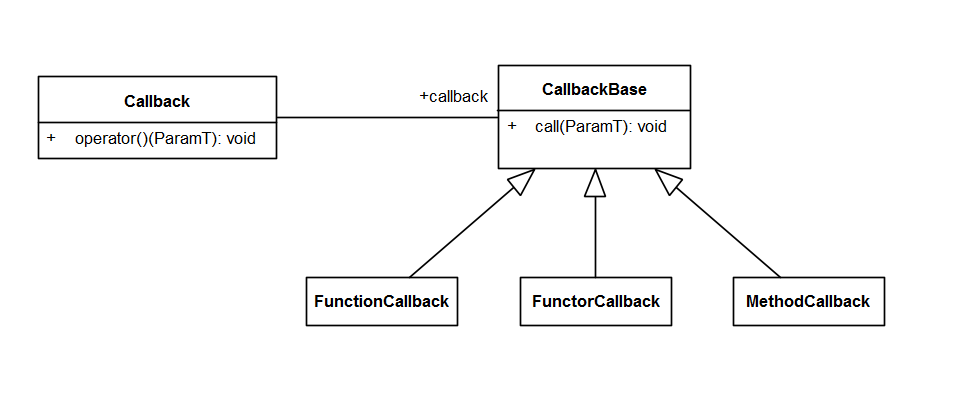
\includegraphics[width=.7\textwidth]{callback_metamodel.png}
\end{center}

\paragraph*{\emph{CallbackBase}}

Fange mit der Klasse \emph{CallbackBase} an.
Damit man beim Aufrufen des Callbacks einen Parameter übergeben kann, füge \emph{call()} einen Parameter vom Typ \emph{ParamT} hinzu, wobei \emph{ParamT} ein Template-Pameter von \emph{CallbackBase} sein soll. Der Klassenrumpf lautet also

\begin{lstlisting}
template<class ParamT>
class CallbackBase {
public:
	...
	virtual void call(ParamT t) = 0;
};
\end{lstlisting} 

Falls ein Callback eigentlich mehrere Parameter erfordert, müssen diese entsprechend in ein Containerobjekt gepackt werden.
Generische Callback-Wrapper mit variabler Parameteranzahl sind zwar möglich, würden aber den Rahmen dieses Praktikums sprengen.

\emph{Tipp}: Du kannst diese und alle nachfolgenden Klassen in einem einzigen Header implementieren, weil die Klassen sehr kurz sind und außerdem semantisch stark zusammenhängen.


\item
\textbf{Klasse \emph{FunctionCallback}}:
Implementiere nun die erste Unterklasse \emph{template<class ParamT> FunctionCallback}, die von \emph{CallbackBase<ParamT>} erbt.  \emph{FunctionCallback} soll einen entsprechenden Funktionszeiger als Attribut besitzen, der bei der Konstruktion initialisiert wird.
Ebenso soll \emph{call(ParamT t)} implementiert werden, wo der gespeicherte Funktionszeiger mit dem gegebenen Argument aufgerufen wird. \\

Teste deine Implementierung.
Lasse \emph{hanoi()} einen Zeiger auf \emph{CallbackBase} nehmen, übergebe aber die Adresse eines \emph{FunctionCallback} Objektes.
Du kannst folgende Vorlage verwenden:
\begin{lstlisting}
#include<utility>
typedef std::pair<int, int> intpair;

void hanoi(..., CallbackBase<intpair> *callback) {
	// ...
	callback->call(intpair(a, c));
	// ...
}

int main() {
	// ...
	CallbackBase<intpair> *function = 
	    new FunctionCallback<intpair>(printMovePair);
	hanoi(3,1,2,3, function);
	// ...
}
\end{lstlisting}


\item
\textbf{Klasse \emph{FunctorCallback}}:
Implementiere nun die Unterklasse \emph{template<class ParamT, class ClassT> FunctorCallback}.
Zusätzlich zum Parameter-Typ muss hier auch der Typ der Functor-Klasse angegeben werden.
Speichere das zu verwendende Functor-Objekt als Referenz ab, um Kopien zu vermeiden.
Achte auch im Konstruktor darauf, dass keine Kopien des Funktors gemacht werden.
Teste deine Implementierung! 



\item
\textbf{Klasse \emph{MethodCallback}}:
Implementiere nun die letzte Unterklasse \emph{template<class ParamT, class ClassT> MethodCallback}.
Beachte, dass nun zwei Attribute nötig sind - ein Methodenzeiger und ein Zeiger auf das zu verwendende Objekt.
Teste deine Implementierung.

\emph{Tipp}: Verwende beispielsweise folgende Signatur für den Konstruktor von \emph{MethodCallback}:
\begin{lstlisting}
MethodCallCallback(void(ClassT::*method)(ParamT), ClassT *object)
\end{lstlisting}

\emph{Tipp 2}: Gegeben einen Zeiger \emph{object} auf ein Objekt, einen Zeiger \emph{method} auf eines seiner Methoden und einen Parameter \emph{p} für die Methode, sieht ein Aufruf von \emph{method} wie folgt aus:
\begin{lstlisting}
	(object->*method)(p);
\end{lstlisting}

\item
\textbf{Klasse \emph{Callback}}: 
Wir haben jetzt den Typ des Callbacks vollständig von seiner Verwendung entkoppelt.
Jedoch muss ein Callback-Objekt per Zeiger/Referenz übergeben werden, sodass das dir schon bekannte  Problem der Zuständigkeit für die Zerstörung eines Objekts entsteht.
Außerdem muss man beim Erstellen eines Callbacks explizit den Typ der Unterklasse angeben.
Es wäre also sinnvoll, einen entsprechenden Wrapper zu schreiben, der sich um die Speicherverwaltung von Callbacks kümmert und bei der Konstruktion die passende Unterklasse selbst aussucht.

Schreibe eine Klasse \emph{template<class ParamT> Callback}, die einen Smart Pointer auf ein \emph{CallbackBase}-Objekt als Attribut hat. Der Smart Pointer soll die Speicherverwaltung übernehmen. Überlade den \emph{operator()}, der den Aufruf einfach an das \emph{CallbackBase}-Objekt hinter dem Smart Pointer weiterleitet. \\

Implementiere nun für jede Callback-Art je einen Konstruktor, der eine Instanz der entsprechenden Unterklasse erzeugt und in dem Smart Pointer speichert.
Der erste Konstruktor soll also einen Funktionszeiger entgegennehmen und ein \emph{FunctionCallback} instanziieren.
Der zweite Konstruktor soll eine Referenz auf ein Funktor-Objekt erwarten und  \emph{FunctorCallback} instanziieren, und der dritte entsprechend ein \emph{MethodCallback}.
Beachte, dass die beiden letztgenannten Konstruktoren selbst Template-Methoden sind, da die \emph{Callback}-Klasse nur an den Parameter-Typ gekoppelt ist.\\

Teste deine Implementierung in Zusammenhang mit der \emph{hanoi}-Funktion. Du kannst das \emph{Callback}-Objekt auch per Wert übergeben, da intern nur Zeiger kopiert werden. 

\end{enumerate}

\textbf{Nachwort}:
Für produktive C++-Programme bietet Boost fertige Funktionen und Klassen, um Callbacks zu realisieren, z.B. \emph{boost::function<...>} und \emph{boost::bind()}\footnote{\url{http://www.boost.org/doc/libs/1_55_0/doc/html/function.html}}. Diese können mit beliebiger Anzahl von Parametern umgehen und beinhalten viele weitere Features.



\section{STL Container} 
In dieser Aufgabe werden wir den Umgang mit den Containern \emph{std::vector} und \emph{std::list} aus der Standard Template Library üben.
Es ist sinnvoll, wenn du während der Übung eine C++-Referenz zum Nachschlagen bereithältst, z.B. \url{http://www.cplusplus.com/}.
Schaue dir auch die Vorlesungsfolien genau an, da diese nützliche Codebeispiele enthalten.

Die Klasse \emph{std::list} stellt eine verkettete Liste dar, bei der man an beliebiger Stelle Elemente effizient löschen und hinzufügen kann. \emph{std::vector} stellt ähnliche Funktionen bereit, allerdings liegen hier die Elemente in einem einzigen, zusammenhängenden Speicherbereich, der neu alloziert und kopiert werden muss, wenn seine aktuelle Kapazität überschritten wird.
Auch müssen viele Elemente verschoben werden, wenn der Vektor in der Mitte oder am Anfang modifiziert wird.
Der große Vorteil von \emph{std::vector} ist der \emph{wahlfreie Zugriff}, d.h. man kann auf beliebige Elemente mit konstantem Aufwand zugreifen.


\begin{enumerate}
\item 
Schreibe zunächst eine Funktion \emph{template<class T> void print(const T \&t)}, die beliebige STL-Container auf die Konsole ausgeben kann, die Integer speichern und Iteratoren unterstützen.
Nutze dazu die Funktion \emph{copy()} sowie die Klasse \emph{ostream\_iterator<int>}, um den entsprechenden \emph{OutputIterator} zu erzeugen.

\item
Lege ein \emph{int}-Array an und initialisiere es mit den Zahlen 1 bis 5.
Lege nun einen \emph{vector<int>} an und initialisiere ihn mit den Zahlen aus dem Array.

\item
Lege eine Liste \emph{list<int>} an und initialisiere diese mit dem zweiten bis vierten Element des Vektors.
\emph{Tipp}: Du kannst auf Iteratoren eines Vektors (genauso wie auf Zeiger) Zahlen addieren, um diese zu verschieben.

\item
Füge mittels \emph{list<T>::insert()} das letzte Element des Vektors an den Anfang der Liste hinzu.

\item
Lösche alle Elemente des Vektors mit einem einzigen Methodenaufruf.

\item
Mittels \emph{remove\_copy\_if()} kann man Elemente aus einem Container in einen anderen kopieren und dabei bestimmte Elemente löschen lassen.
Nutze diese Funktion, um alle Elemente, die kleiner sind als 4, aus der Liste in den Vektor zu kopieren. Beachte, dass \emph{remove\_copy\_if()} keine neuen Elemente an den Container anhängt, sondern lediglich Elemente von der einen Stelle zur anderen elementweise durch Erhöhen des \emph{OutputIterator} kopiert.

Deshalb kannst du \emph{vec.end()} \textbf{nicht} als \emph{OutputIterator} nehmen, da dieser "{}hinter"{} das letzte Element zeigt und weder dereferenziert noch inkrementiert werden darf. Nutze stattdessen die Methode \emph{back\_inserter()}, um einen Iterator zu erzeugen, der neue Elemente an den Vektor anhängen kann.
\end{enumerate}

\section{Exceptions}
Ähnlich wie in Java können Fehler in C++ mittels Exceptions signalisiert werden.

\begin{lstlisting}
try {
	...
	throw <Type>;
} catch(<Type1> <param name>) {
	...
} catch(<Type2> <param name>) {
	...
}
...
\end{lstlisting} 

Es gibt jedoch einige Unterschiede zur Fehlerbehandlung in Java.
Das aus Java bekannte \emph{finally}-Konstrukt existiert in C++ nicht.
Außerdem kann jede Art von Wert geworfen werden -- sowohl Objekte als auch primitive Werte wie z.B. \emph{int}.
In der Praxis wird es jedoch empfohlen, den geworfenen Wert von \emph{std::exception} abzuleiten oder eine der existierenden Klassen aus der Standardbibliothek zu nutzen. \\

Im Gegensatz zu Java kann man Objekte nicht nur \emph{by-Reference} sondern auch \emph{by-Value} werfen und fangen. In diesem Fall wird das geworfene Objekt nach der Behandlung im \textbf{catch}-Block automatisch zerstört. Wenn es \emph{by-Value} gefangen wird, wird das geworfene Objekt kopiert, ähnlich wie bei einem Funktionsaufruf. Beispiel:

\begin{lstlisting}
// 1. Catch by value
try {
	throw C(); // create new object of class C and throw it 
} catch(C c) { // catch c by value => a copy of c is created when catching
	...
}

// 2. Catch by reference
try {
	throw C(); // create new object of class C and throw it 
} catch(const C &c) { // catch c by reference, no copy is created
	...
}
\end{lstlisting} 

In der Praxis hat es sich durchgesetzt, \emph{by-Value} zu werfen und \emph{by-const-Reference} zu fangen.

\begin{enumerate}
\item 
Erstelle eine Klasse \emph{C} und implementiere einen Konstruktor, einen Copy-Konstruktor und einen Destruktor.
Versehe diese mit Ausgaben auf der Konsole, so dass der Lebenszyklus während der Ausführung ersichtlich wird.

\item 
Experimentiere mit Exceptions.
Probiere insbesondere die beiden o.g. Fälle aus und beobachte die Ausgabe. 
Wann wird ein Objekt erstellt/kopiert/gelöscht? 
Teste auch, was passiert, wenn du mehrere \emph{catch}-Blöcke erstellst und sich diese nur in der Übergabe unterscheiden (Wert/Referenz). Welcher von ihnen wird aufgerufen?
Spielt die Reihenfolge eine Rolle?

\item
Füge der Klasse \emph{List} aus \ref{sec:list} (oder dem Array aus \ref{sec:array}) Bereichsprüfungen hinzu.
Schreibe die Methoden \emph{insertElementAt()}, \emph{getNthElement()} und \emph{deleteAt()} so um, dass eine Exception geworfen wird, falls der angegebene Index die Größe der Liste überschreitet. 
Nimm dafür die Klasse \emph{std::out\_of\_range} aus dem \emph{stdexcept} Header.

\item
Teste deine Implementierung.
Provoziere eine Exception, indem du falsche Indices angibst, und fange die Exception als \emph{const} Referenz ab. Du kannst die Methode \emph{what()} benutzen, um an den Nachrichtentext der Exception zu gelangen.

\end{enumerate}


\section{C Einführung}
In den nächsten Tagen werden wir Programme für eine Embedded Plattform in C entwickeln. 
Da C++ aus C entstand, sind viele Features von C++ nicht in C enthalten. Im Folgenden sollen die Hauptunterschiede verdeutlicht werden.

\begin{itemize}
	\item Kein OO-Konzept, keine Klassen, nur Strukturen (\emph{struct}).
	\item Keine Templates
	\item Keine Referenzen, nur Zeiger und Werte
	\item Kein \emph{new} und \emph{delete}, sondern \emph{malloc()} und \emph{free()} (\verb|#include <stdlib.h>|)
	\item Je nach Sprachstandard müssen Variablen am Anfang der Funktion deklariert werden (Standard-Versionen $<$ C99)
	\item Parameterlose Funktionen müssen \emph{void} als Parametertyp haben, leere Klammern () bedeuten, dass beliebige Argumente erlaubt sind.
	\item Keine Streams, stattdessen \emph{(f)printf} zur Ausgabe auf Konsole und in Dateien (\verb|#include <stdio.h>|)
	\item Kein \emph{bool} Datentyp, stattdessen wird 0 als \emph{false} und alle anderen Zahlen als \emph{true} gewertet
	\item Keine Default-Argumente
	\item Keine \emph{std::string} Klasse, nur \emph{char}-Arrays, die mit dem Nullbyte (\verb|'\0'|) abgeschlossen werden.
	\item Keine Namespaces
\end{itemize}

Da einige dieser Punkte sehr entscheidend sind, werden wir auf diese im Detail eingehen.

\begin{itemize}
	\item[] \textbf{Kein OO-Konzept}\\\\
	In C gibt es keine Klassen, weshalb die Programmierung in C eher Pascal statt C++ ähnelt.
	Stattdessen gibt es Strukturen (\textbf{struct}), die mehrere Variablen zu einem Datentyp zusammenfassen, was vergleichbar mit Records in Pascal oder -- allgemein -- mit Klassen ohne Methoden und ohne Vererbung ist.\\
	
	Die Syntax dafür lautet
	\begin{lstlisting}
	struct MyStruct {
	<Type1> <Name11>, <Name12>, ...;
	<Type2> <Name21>, <Name22>, ...;
	};
	\end{lstlisting} 
	
	Zum Beispiel
	\begin{lstlisting}
	struct Point {
	int x;
	int y;
	};
	\end{lstlisting}
	
	Die Sichtbarkeit aller Attribute ist automatisch \emph{public}. \\
	
	Um den definierten \textbf{struct} als Datentyp zu verwenden, muss man zusätzlich zum Namen das Schlüsselwort \textbf{struct} angeben:
	
	\begin{lstlisting}
	void foo(struct Point *p) {
	...
	}
	...
	int main(void) {
	struct Point point;
	foo(&point);
	}
	\end{lstlisting}
	
	Um den zusätzlichen Schreibaufwand zu vermeiden, wird in der Praxis oft ein \textbf{typedef} auf den \textbf{struct} definiert:
	
	\begin{lstlisting}
	typedef struct Point Point_t;
	...
	Point_t point;
	\end{lstlisting}
	
	Man kann die Deklaration eines \textbf{struct} auch direkt in den \textbf{typedef} einbauen:
	\begin{lstlisting}
	typedef struct {
	int x;
	int y;	
	} Point;
	\end{lstlisting}
	
	\item[] \textbf{Kein \emph{new} und \emph{delete}}
	
	Anstelle von \emph{new} und \emph{delete} werden die Funktionen \emph{malloc} und \emph{free} verwendet, um Speicher auf dem Heap zu reservieren. 
	Diese sind im Header \emph{stdlib.h} deklariert.
	
	\begin{lstlisting}
	#include <stdlib.h>
	Point *points = malloc(10 * sizeof(Point)); // reserve memory for 10 points
	// ...
	free(points);
	\end{lstlisting} 
	
	\item[] \textbf{Ausgabe auf Konsole per \emph{printf}}
	
	Um Daten auf der Konsole auszugeben, kann die Funktion \emph{printf} verwendet werden.
	\emph{printf()} nimmt einen Format-String sowie eine beliebige Anzahl weiterer Argumente entgegen.
	Der Format-String legt fest, wie die nachfolgenden Argumente ausgegeben werden.
	Mittels \textbackslash n kann man einen Zeilenvorschub erzeugen. Um \emph{printf()} zu nutzen, muss der Header \emph{stdio.h} eingebunden werden. 
	
	\begin{lstlisting}
	#include <stdio.h>
	printf("Hallo Welt\n"); // Hallo Welt + neue Zeile ausgeben
	
	int i;
	printf("i = %d\n", i);  // Integer ausgeben
	printf("i = %3d\n", i); // Integer ausgeben, auf drei Stellen auffüllen
	
	int i;
	char c;
	printf("c = %c, i = %d\n", c, i); // Zeichen und Integer ausgeben
	\end{lstlisting} 
	
	Weitere Möglichkeiten von \emph{printf()} findest du unter \url{http://www.cplusplus.com/reference/cstdio/printf/}.
	
\end{itemize}

Zum Abschluss noch ein paar Aufgaben, um mit C etwas warm zu werden:

\begin{enumerate}
	\item 
	Schreibe ein C-Programm, welches alle geraden Zahlen von 0 bis 200 formatiert ausgibt. 
	Die Formatierung soll entsprechend dem Beispiel erfolgen:
	\begin{lstlisting}
	2   4   6   8  10
	12  14  16  ...
	\end{lstlisting}
	
	\item Versuche, beliebige (einfache) Programme der vergangenen Tage in reinem C auszudrücken (Schwierigkeitsgrad sehr unterschiedlich!).
\end{enumerate}

\section{Eigene Arrays (optional)}
\label{sec:array}

Nachdem du bei unseren Übungen zu Arrays gesehen hast, dass es störend ist, wenn man die Größe eines Arrays immer getrennt zu den gespeicherten Daten verwalten muss, ist ein sinnvoller Schritt, eine eigene Array-Klasse zu implementieren, die Daten und Größe des Arrays zusammen speichert.

Eine möglicher Anwendungsfall sieht so aus:

\begin{lstlisting}
#include "Array.h"
#include <iostream>
#include <string>

using namespace std;

template<class T>
void printFirst(const Array<T> &array) {
    cout << array[0] << endl;
}

int main(int argc, char **argv) {
    Array<std::string> stringArray(10);
    stringArray[0] = "Hello World";

    printFirst(stringArray);

    return 0;
}
\end{lstlisting}

\emph{Hinweise}:
\begin{itemize}
\item
Überlege dir, welche Operatoren/Methoden das obige Code-Beispiel von Array verlangt.
Unter anderem musst du jeweils einen \emph{const} und einen nicht-\emph{const} \emph{operator[]} implementieren.

\item
Du kannst auch Exceptions (z.B. \emph{std::out\_of\_range} aus \emph{<stdexcept>}) verwenden, um falsche Indices korrekt abzufangen.

\item
Eine fortgeschrittene Übung ist es, Iteratoren oder \emph{operator+} für das Array bereitszustellen, sodass du z.B. die Funktion \emph{std::copy} aus der STL verwenden kannst, um ein Array zu kopieren:
\begin{lstlisting}
#include <algorithm> // copy
#include <iterator> // back_inserter
#include <vector>
// ...
Array<int> array(10);
std::vector<int> vector;
std::copy(array, array + 4, std::back_inserter(vector));
\end{lstlisting}

\item
Diese Idee ist natürlich nicht neu.
Seit C++11 gibt es eine Array-Implementierung in der C++-Standardbibliothek (\emph{std::array}\footnote{\url{http://www.boost.org/doc/libs/1_55_0/doc/html/array.html}}).
Du findest die gleiche Klasse auch als \emph{boost::array} in Boost.
Wenn du damit experimentieren willst, mussst du die Compiler-Unterstützung für C++11 einschalten.
Gehe dazu in die Projekteigenschaften (\emph{Rechtsklick} $\to$ Properties) und setzte unter \emph{C/C++-Build/Settings/GCC C++ Compiler/Dialect} das Feld \emph{Language Standard} auf \emph{ISO C++11}.
\end{itemize}




\section{Makefiles (optional)}

In dieser Übung erkunden wir, wie man Makefile-Projekte in Eclipse aufbaut.
Wir bauen dafür einen Teil unseres Aufzugsimulators nach, um zu sehen, wo die Herausforderungen in echten Projekten mit Makefiles gelöst werden können.

\begin{enumerate}
\item\textbf{Projekt anlegen}
Öffne \emph{File $\to$ New $\to$ C++ Project} und wähle \textbf{Project type: Makefile project/Empty Project}.
Wähle als \textbf{Toolchain} \textbf{MinGW GCC} aus und suche dir einen Projektnamen aus.

Das erzeugte Projekt ist ziemlich leer.
Lege zunächst ein Makefile an über \textbf{File $\to$ New $\to$ Other\dots} und dann \textbf{File}.

Eclipse erwartet, dass das Makefile ein Target mit dem Namen \emph{all} hat.
Um unser Projekt zu testen, geben wir zunächst eine einfache Meldung auf der Kommandozeile aus.
Lege nun das Target \emph{all} an und füge den folgenden Befehl an (Vergiss dabei nicht den Tab vor jedem Befehl!):
\begin{lstmake}
all:	
	@echo "Running all..."
\end{lstmake}

Wenn du jetzt \emph{Build} aufrufst, sollte in der \emph{Console View} in etwa Folgendes erscheinen:
\begin{verbatim}
18:17:25 **** Incremental Build of configuration Default for project ExerciseMakefileProject ****
make all 
Running all...

18:17:26 Build Finished (took 140ms)
\end{verbatim}

\item\textbf{Erster Compilevorgang}

Jetzt ist es an der Zeit, ein Programm mittels \emph{make} zu kompilieren.
Lege dazu eine C++-Sourcedatei \emph{main.cpp} mit einer \emph{main}-Funktion an, die etwas sinnvolles ausgibt.

Entgegen unserer bisherigen Erfahrung musst du nun manuell in das Makefile eintragen, dass \emph{main.cpp} gebaut werden soll.
Ersetze die Dummy-Ausgabe daher durch einen Compiler-Aufruf an \emph{g++}:
\begin{lstmake}
all:
	g++ -o main.exe main.cpp
\end{lstmake}

Wenn du jetzt \emph{Build} aufrufst, wird dein Programm kompiliert und als \emph{main.exe} im Projekthauptverzeichnis abgelegt.

\item\textbf{Klasse \emph{Building}}
Jetzt fügen wir die Klasse \emph{Building} zu unserem Projekt hinzu, die allerdings nur minimale Funktionalität bietet:

\begin{minipage}[t]{.45\textwidth}
\begin{lstlisting}
/*
* File: Building.h
*/
#ifndef BUILDING_H_
#define BUILDING_H_

#include <string>

class Building {
public:
    Building(unsigned int numFloors);
    const std::string toString() const;
private:
    unsigned int numFloors;
};
#endif
\end{lstlisting}
\end{minipage}
\begin{minipage}[t]{.45\textwidth}
\begin{lstlisting}
/*
* File: Building.cpp
*/
#include "Building.h"

#include <string>
#include <sstream>

using namespace std;

Building::Building(unsigned int numFloors) :
    numFloors(numFloors) {}

const std::string Building::toString() const{
    stringstream output;
    output << "A building with " 
           << this->numFloors 
           << " floors\n";
    return output.str();
}
\end{lstlisting}
\end{minipage}

Erzeuge in \emph{main} eine zweistöckige Instanz von \emph{Building} und gib diese mittels \emph{Building::toString} auf der Konsole aus.

Damit das Projekt kompiliert, muss auch \emph{Building} im Makefile eingetragen werden.
Passe dazu den Compileraufruf an:
\begin{lstmake}
all:
    g++ -o main.exe main.cpp Building.cpp
\end{lstmake}

Wenn du das Projekt gebaut hast, sollte auf der Konsole eine Ausgabe deines Gebäudes erscheinen.

\item\textbf{Compiler-Aufrufe auslagern}
In der Vorlesung haben wir gesehen, dass \emph{make} anhand der Zeitstempel von Dateien dazu in der Lage ist, zu erkennen, wann ein Programmteil neu gebaut werden muss.
Aktuell nutzen wir diese Möglichkeit noch nicht:
Egal ob wir \emph{main.cpp}, \emph{Building.cpp} oder \emph{Building.h} verändert haben, immer wird das gesamte Projekt neu gebaut.
In diesem Schritt zerlegen wir die Abhängigkeiten zu den einzelnen Dateien.

Mache das Target \emph{all} jetzt abhängig von den Objektdateien \emph{main.o} und \emph{Building.o} und erzeuge für jede Objektdatei ein eigenes Ziel, welches diese baut (Das Flag \emph{-c} sorgt dafür, dass die Sourcedateien nur kompiliert, aber nicht gelinkt werden).
\begin{lstmake}
all: main.o Building.o
	g++ -o main.exe main.o Building.o

main.o: main.cpp
	g++ -c -o main.o main.cpp

Building.o: Building.cpp
	g++ -c -o Building.o Building.cpp
\end{lstmake}

Baue das Projekt nun erneut, du solltest drei Aufrufe von \emph{g++} sehen:
\begin{verbatim}
make all 
g++ -c -o main.o main.cpp
g++ -c -o Building.o Building.cpp
g++ -o main.exe main.o Building.o
\end{verbatim}
Baust du das Projekt nun erneut, so wird nur noch der Linker aufgerufen:
\begin{verbatim}
make all 
g++ -o main.exe main.o Building.o
\end{verbatim}

\item\textbf{Linker-Aufruf auslagern}
Wie können wir diesen an sich unnötigen Aufruf ebenfalls noch loswerden?
Eine Lösung ist es, das Target \emph{all} von \emph{main.exe} abhängig zu machen und ein neues Ziel \emph{main.exe} zu definieren:
\begin{lstmake}
all: main.exe

main.exe: main.o Building.o
	g++ -o main.exe main.o Building.o

# ...
\end{lstmake}

Wenn du das Projekt jetzt baust, erhältst du erfreulicherweise die Rückmeldung, dass nichts zu tun ist:
\begin{verbatim}
make all 
make: Nothing to be done for `all'.
\end{verbatim}

\item\textbf{Inkrementelles Bauen}
Wir erproben jetzt, wie sich Veränderungen an einer der drei Dateien auf die Ausführung von \emph{make} auswirken.
Mache nacheinander kleine Änderungen -- das können auch Kommentare sein -- an den Dateien \emph{main.cpp}, \emph{Building.h} und \emph{Building.cpp} und baue das Projekt nach jeder Änderung.

Dir fällt auf, dass Änderungen an \emph{Building.h} von \emph{make} nicht bemerkt werden; die Datei taucht ja nirgendwo explizit im Makefile auf.

Wir sehen uns jetzt an, welche Tragweite dieses Problem haben kann.


\item\textbf{Header als Abhängigkeiten}
Du hast kennengelernt, dass man Implementierungen auch \emph{inline} in einem Header machen kann, zum Beispiel wenn diese klein sind.

Bewege \emph{toString} nun nach \emph{Buidling.h}:
\begin{lstlisting}
#include <sstream>
// ...
inline const std::string toString() const{

    std::stringstream output;
    output << "A building with " << this->numFloors << " floors\n";
    return output.str();
}
\end{lstlisting}

Baue das Projekt; es kompiliert nicht! Warum? Genau aus dem Grund, dass \emph{make} das Header-File nicht \glqq kennt\grqq{}.
Jetzt gibt es im Projekt keine Definition von \emph{toString} wie uns der Linker auch mitteilt:
\begin{verbatim}
main.o:main.cpp:(.text+0x5c): undefined reference to `Building::toString() const'
collect2: ld returned 1 exit status
\end{verbatim}

Das Problem lässt sich lösen, indem wir im Makefile angeben, dass \emph{main.o} nicht nur abhängig von \emph{Building.cpp}, sondern auch von \emph{Building.h} ist:
\begin{lstmake}
# ...
main.o: main.cpp Building.h
	g++ -c -o main.o main.cpp
# ...
\end{lstmake}

Ist das eine schöne Lösung?
Sicherlich nicht, denn ab sofort müssten wir manuell alle Header ins Makefile eintragen, die wir per \emph{\#include} in eine Sourcedatei einbinden.
Schlimmer noch: Wir müssten über rekursive Includes Bescheid wissen, z.B. wenn \emph{Building.h} einen anderen veränderlichen Header wie \emph{Floor.h} einbindet.

Glücklicherweise hilft uns \emph{g++} bei diesem Problem.

\item\textbf{Header automatisch als Abhängigkeiten deklarieren}

Wir automatisieren jetzt die Erkennung von Headern als Abhängigkeiten.
Lösche dazu die Abhängigkeit \emph{Building.h} des Targets \emph{main.o} und füge in den Compiler-Aufrufen die Parameter \emph{-MMD -MP} hinzu.
Binde außerdem die Dateien \emph{Building.d} und \emph{main.d} ein wie unten dargestellt:
\begin{lstmake}
all: main.exe

main.exe: main.o Building.o
	g++ -o main.exe main.o Building.o

main.o: main.cpp
	g++ -c -MMD -MP -o main.o main.cpp

Building.o: Building.cpp
	g++ -c -MMD -MP -o Building.o Building.cpp

-include Building.d main.d
\end{lstmake}

Um den Effekt dieser Lösung zu sehen, müssen wir alle generierten Dateien löschen (\emph{main.exe, Building.h, Building.cpp}).
Das anschließende Bauen sollte nun funktionieren.

Der Trick ist, dass \emph{g++} beim Kompilieren für jede Sourcedatei ein Makefile generiert, das dessen eingebundene Header als Abhängigkeiten enthält (\emph{main.d, Building.d}).

Wenn du jetzt Änderungen an der \emph{toString}-Methode durchführst, werden diese anhand des Zeitstempels von \emph{Building.h} erkannt.




\item\textbf{Target \emph{clean}}

Bisher mussten wir hin und wieder die kompilierten Dateien manuell löschen, wenn wir unser Projekt neu bauen wollten.
Diese Aufgabe lässt sich mittels \emph{make} ebenfalls automatisieren.

Lege dazu ein neues Target \emph{clean} ohne Abhängigkeiten an und füge einen entsprechenden Löschbefehl ein:
\begin{lstmake}
clean:
	rm -rf main.o Building.o main.d Building.d main.exe

.PHONY: clean
\end{lstmake}
Das Spezial-Target \emph{.PHONY} dient dazu, \emph{make} zu signalisieren, dass \emph{clean} keine Datei ist, die gebaut werden soll.
Würden wir dieses Target auslassen und eine Datei mit Namen \emph{clean} erzeugen, würde \emph{make} die Regel nie ausführen, weil die Datei ja existiert und keine Abhängigkeiten besitzt.
Probier' es ruhig aus!

Um \emph{clean} ausführen zu können, öffne die \textbf{Make Target} View über \textbf{Window $\to$ Show View $\to$ Other\dots $\to$ Make/Make Target}.

Klicke rechts auf dein Projekt und wähle \textbf{New\dots}.
Gib in das Feld \textbf{Make Target} \textbf{\emph{clean}} ein und lasse den Rest unverändert.
Unter deinem Projekt wurde nun ein neuer Knoten mit dem Namen \emph{clean} eingefügt.
Wenn du diesen doppelt anklickst, wird das Target \emph{clean} ausgeführt.

Lege dir nun auch ein ausführbares Target für \emph{all} an.





\item\textbf{Generisches Compiler-Target}
Dir ist sicherlich aufgefallen, dass wir zwei Targets haben, die mehr oder weniger identisch sind: \emph{main.o} und \emph{Building.o}.

\emph{make} bietet für solche Situationen generische Regeln an, die mittels Wildcards beschrieben werden.

Ersetze die beiden spezifischen Targets durch folgendes generisches:
\begin{lstmake}
%.o: %.cpp
	g++ -MMD -MP -c $< -o $@
\end{lstmake}
Die etwas kryptischen Ausdrücke \emph{\$<} und \emph{\$@} werden durch die aktuelle Abhängigkeit und Target ersetzt.

Lösche alle automatisch generierten Dateien (\emph{make clean}) und baue das Projekt neu.





\item\textbf{Variablen in make}

Im Moment sieht unser Makefile in etwa so aus:
\begin{lstmake}
all: main.exe

main.exe: main.o Building.o
	g++ -o main.exe main.o Building.o

%.o: %.cpp
	g++ -MMD -MP -c $< -o $@

-include Building.d main.d

clean:
	rm -rf main.o Building.o main.d Building.d main.exe
	
.PHONY: clean
\end{lstmake}

Dir ist sicherlich eine andere Form der Redundanz aufgefallen:
Noch immer haben wir die Tatsache, dass es im Moment zwei Sourcedateien gibt, an unterschiedlichen Stellen im Makefile festgelegt.
Wenn wir nun als nächstes die \emph{Floor}-Klasse entwerfen, müssten wir diese hinzufügen
\begin{compactitem}
\item als Abhängigkeit von \emph{main.exe},
\item zum Linker-Aufruf in \emph{main.exe},
\item in der \emph{-include}-Direktive und
\item im Lösch-Target, und das gleich doppelt!
\end{compactitem}
Das ist natürlich immer noch ziemlich fehleranfällig.

Wir würden also gerne nur an \emph{einer} Stelle definieren, welche Sourcedateien Teil unseres Projektes sind.

Da die Sourcedateien nirgendwo im Makefile auftreten, fangen wir mit den Object-Dateien an.
Lege am Anfang des Makefiles eine Variable mit dem Inhalt '\emph{main.o Building.o}' und ersetze das Auftreten der beiden Object-Dateien mit dieser Variablen:
\begin{lstmake}
objFiles=main.o Building.o

all: main.exe

main.exe: $(objFiles)
	g++ -o main.exe $(objFiles)
	
# and so on...
\end{lstmake}
\emph{Tipp}: Eclipse bietet für Variablennamen automatische Vervollständigung an (\emph{Ctrl+Space}).

Wiederhole die Prozedur für die Dependency-Dateien ('\emph{dFiles=main.d Building.d}') und das ausführbare Programm ('\emph{programName=main.exe}').
Lasse dein Programm zwischendurch immer wieder vollständig neu bauen, um sicherzustellen, dass nichts kaputt geht.

Am Ende sollte dein Makefile in etwa so aussehen:
\begin{lstmake}
programName=main.exe
objFiles=main.o Building.o
dFiles=main.d Building.d

all: $(programName)

$(programName): $(objFiles)
	g++ -o $(programName) $(objFiles)

%.o: %.cpp
	g++ -MMD -MP -c $< -o $@

-include $(dFiles)

clean:
	rm -rf $(objFiles) $(dFiles) $(programName) 
	
.PHONY: clean
\end{lstmake}
%$ for syntax highlighting

Wie wir die verbliebene Redundanz auflösen, sehen wir in der nächsten Teilaufgabe.

\item\textbf{Wildcard-Ausdrücke}

Die beiden Variablen \emph{objFiles} und \emph{dFiles} sind strukturell ähnlich -- wieder etwas, das wir loswerden wollen.
Außerdem wäre es doch viel schöner, an einer Stelle die Sourcedateien zu definieren, oder?

Lege dazu eine neue Variable \emph{sourceFiles} mit den beiden Sourcedateien an.
Der folgende Snippet zeigt, wie man nun mittels Suffix-Ausdrücken die anderen beiden Variablen erzeugt:
\begin{lstmake}
programName = main.exe
sourceFiles = main.cpp Building.cpp
objFiles   = $(sourceFiles:.cpp=.o)
dFiles     = $(sourceFiles:.cpp=.d)

# ...
\end{lstmake}

Es geht sogar noch allgemeiner:
Du kannst per regulärem Ausdruck definieren, dass \emph{alle} Sourcedateien im aktuellen Ordner verwendet werden sollen, indem du \emph{sourceFiles} wie folgt definierst:

\begin{lstmake}
sourceFiles=$(wildcard ./*.cpp)
\end{lstmake}
%$ for syntax highlighting

\end{enumerate}

Das Produkt unserer Bemühungen in dieser Aufgabe ist ein Makefile, das unabhängig davon ist, wie viele Sourcedateien du im aktuellen Verzeichnis hältst und wie sie genau heißen -- wichtig ist nur die Endung \emph{cpp}.

Hier nochmal das vollständige Makefile:
\begin{lstmake}
programName=main.exe
sourceFiles=$(wildcard ./*.cpp)
objFiles=$(sourceFiles:.cpp=.o)
dFiles=$(sourceFiles:.cpp=.d)

all: $(programName)

$(programName): $(objFiles)
	g++ -o $(programName) $(objFiles)

%.o: %.cpp
	g++ -MMD -MP -c $< -o $@

-include $(dFiles)

clean:
	rm -rf $(objFiles) $(dFiles) $(programName)

.PHONY: clean
\end{lstmake}

\textbf{Nachwort}:

Wenn du diese Aufgabe durchgestanden hast, hast du einen Eindruck davon erhalten, wie gut man sich auskennen muss, um ein Projekt mittels \emph{make} zu managen;
dabei sind dies hier nur äußerst wenige der Möglichkeiten, die \emph{make} bietet\footnote{Für einen besseren Eindruck, sieh dir die Doku an: \url{https://www.gnu.org/software/make/manual/html_node/index.html}}.

In der Praxis existieren Build-Tools, die eine wesentlich besser zu verstehende Beschreibungssprache verwenden und daraus Makefiles generieren.
Beispiele sind \emph{cmake}\footnote{\url{http://www.cmake.org/cmake/help/cmake_tutorial.html}} oder \emph{qmake}\footnote{\url{http://qt-project.org/doc/qt-4.8/qmake-tutorial.html}} (Bestandteil von Qt).


\end{document}
